% This LaTeX was auto-generated from MATLAB code.
% To make changes, update the MATLAB code and export to LaTeX again.

\documentclass{article}

\usepackage[utf8]{inputenc}
\usepackage[T1]{fontenc}
\usepackage{lmodern}
\usepackage{graphicx}
\usepackage{color}
\usepackage{hyperref}
\usepackage{amsmath}
\usepackage{amsfonts}
\usepackage{epstopdf}
\usepackage[table]{xcolor}
\usepackage{matlab}

\sloppy
\epstopdfsetup{outdir=./}
\graphicspath{ {./topt_p5_images/} }

\matlabhastoc

\begin{document}

\label{T_B44F81CE}
\matlabtitle{\textbf{PRACTICE 5 - OPTIMIZATION TECHNIQUES}}

\begin{par}
\begin{flushleft}
\textbf{Andrés Herencia y Antonio Fernández}
\end{flushleft}
\end{par}

\begin{par}
\begin{flushleft}
\textbf{MUTECI 2023-2024}
\end{flushleft}
\end{par}

\matlabtableofcontents{Table of Contents}

\label{H_49734934}
\matlabheading{\textbf{Exercise 1}}

\begin{par}
\begin{flushleft}
Using the data from the file \texttt{datos\_regr\_orto.txt,} the following is requested: 
\end{flushleft}
\end{par}

\begin{par}
\begin{flushleft}
    a) Propose an optimization model to solve the orthogonal regression problem for the model $y=\beta_0 +\beta_1 x+\beta_2 x^2$.
\end{flushleft}
\end{par}

\begin{par}
\begin{flushleft}
    b) Solve it using the appropriate software.
\end{flushleft}
\end{par}

\begin{par}
\begin{flushleft}
    c) Compare the result with the standard regression model (a graphical comparison is acceptable).
\end{flushleft}
\end{par}


\label{H_DF7E7F40}
\matlabheadingtwo{Solution}

\label{H_DE9148FD}
\matlabheadingthree{a) Propose an optimization model to solve the orthogonal regression problem for the model $y=\beta_0 +\beta_1 x+\beta_2 x^2$.}

\begin{par}
\begin{flushleft}
a) First of all, we will read our data:
\end{flushleft}
\end{par}

\begin{matlabcode}
clear
cd('C:\Users\andre\Documents\UNIVERSIDAD\MUTECI\BLOQUE 2\TOPT\lab\P5\')
clc

fid = fopen('datos_regr_orto.txt', 'r');
fgetl(fid);
data = textscan(fid, '%f %f');
fclose(fid);
x = data{1}; x2 = x.^2;n = length(x);
X = [ones(n,1),x,x2];
y = data{2};
data = [y,x]
\end{matlabcode}
\begin{matlaboutput}
data = 6x2    
    4.8000    0.2000
    7.1000    0.9000
    5.3000    2.2000
    1.8000    2.9000
   -2.8000    4.1000
  -10.5000    5.2000

\end{matlaboutput}
\begin{matlabcode}
clc
figure(1)
plot(x,y,'bo')
xlabel('x')
ylabel('y')
title('Original data')
grid on
\end{matlabcode}
\begin{center}
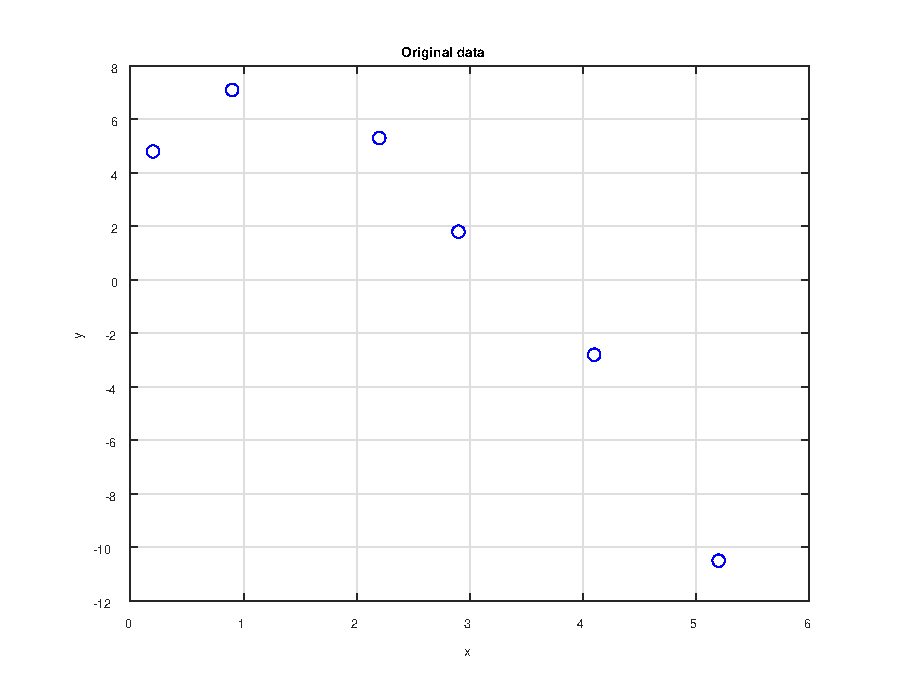
\includegraphics[width=\maxwidth{56.196688409433015em}]{figure_0.eps}
\end{center}

\begin{par}
\begin{flushleft}
We define $\epsilon_i ={Y_i }^* -Y_i$ as the error associated to $Y_i$, and $\delta_i ={X_i }^* -X_i$ as the associated error to each $X_i$, with $i=1,\ldots,n\ldotp$
\end{flushleft}
\end{par}

\begin{par}
\begin{flushleft}
Then, we consider the orthogonal problem to solve an orthogonal regression problem as it follows.
\end{flushleft}
\end{par}

\begin{par}
$$\begin{array}{l}
\min_{\beta ,\epsilon_i ,\delta_i } ~~\sum_{i=1}^n (\epsilon_i^2 +\delta_i^2 )\\
\textrm{such}\;\textrm{to}~~Y_i =f(X_i +\delta_i ;\beta )-\epsilon_i ,~~i=1,\ldots,n.
\end{array}$$
\end{par}

\begin{par}
\begin{flushleft}
If we reordenate the problem substituting $\epsilon_{i\;}$and $\delta_i$ in function of $X_i$ and $Y_i$, we finally obtain:
\end{flushleft}
\end{par}

\begin{par}
$$\min_{\beta^* ,\delta^* } \sum_{i=1}^n \lbrace (f(X_i +\delta_i ;\beta )-Y_i )^2 +\delta_i^2 \rbrace$$
\end{par}

\begin{par}
\begin{flushleft}
And if we substitute for our concrete problem we get:
\end{flushleft}
\end{par}

\begin{par}
$$\min_{\beta^* ,\delta^* } \sum_{i=1}^n \lbrace [\beta_0 +\beta_1 x^* +\beta_2 x^{*2} -Y_i ]^2 +(x^* -x)^2 +(x^{*2} -x^2 )^2 \rbrace$$
\end{par}

\begin{par}
\begin{flushleft}
Where the $*$ symbol represents our estimation.
\end{flushleft}
\end{par}


\label{H_EE595B5D}
\matlabheadingthree{b) Solve it using the appropriate software.}

\begin{par}
\begin{flushleft}
The initial values of the errors associated with $x$ will be the $y$ vector, meanwhile, the $\beta$ coefficients could be the result of making the quadratic regression (this regression can be perform via the \texttt{polyval} command). Then:
\end{flushleft}
\end{par}

\begin{matlabcode}
b2 = polyfit(x,y,2);
O = [b2,x']
\end{matlabcode}
\begin{matlaboutput}
O = 1x9    
   -0.9683    2.0096    5.1102    0.2000    0.9000    2.2000    2.9000    4.1000    5.2000

\end{matlaboutput}
\begin{matlabcode}
orto = @(E) orthogonal_regression(x,y,E);
[error, fval] = fminunc(orto,O)
\end{matlabcode}
\begin{matlaboutput}
Local minimum found.

Optimization completed because the size of the gradient is less than
the value of the optimality tolerance.

<stopping criteria details>
error = 1x9    
    5.1103    2.0095   -0.9682    0.2000    0.9000    2.2000    2.9000    4.1000    5.2001

fval = 2.6135
\end{matlaboutput}
\begin{matlabcode}
beta = error(1:3);
eps = error(4:end);
\end{matlabcode}

\begin{par}
\begin{flushleft}
Finally our orthogonal regression model over $y=\beta_0 +\beta_1 x+\beta_2 x^2$ with 
\end{flushleft}
\end{par}

\begin{par}
$$\left\lbrace \begin{array}{c}
\beta_0 =5.1103\\
\beta_1 =2.0095\\
\beta_2 =-0.9682
\end{array}\right.$$
\end{par}

\begin{matlabcode}
xq = min(x):length(x)/100:max(x);
y_orto = beta(1) + beta(2).*xq + beta(3).*xq.^2;
\end{matlabcode}


\label{H_EB9112E3}
\matlabheadingthree{c) Compare the result with the standard regression model (a graphical comparison is acceptable).}

\begin{par}
\hfill \break
\end{par}

\begin{matlabcode}
X = [ones(length(x),1),x];
b1 = regress(y,X);
Y1 = b1(1) + b1(2).*x;
spl = spline(x,y,xq)
\end{matlabcode}
\begin{matlaboutput}
spl = 1x84    
    4.8000    5.0884    5.3596    5.6137    5.8506    6.0704    6.2730    6.4586    6.6272    6.7788    6.9134    7.0310    7.1317    7.2155    7.2824    7.3325    7.3658    7.3823    7.3820    7.3650    7.3314    7.2810    7.2140    7.1304    7.0301    6.9134    6.7801    6.6303    6.4640    6.2812    6.0821    5.8665    5.6346    5.3864    5.1219    4.8429    4.5517    4.2510    3.9431    3.6307    3.3161    3.0020    2.6908    2.3851    2.0873    1.8000    1.5250    1.2619    1.0093    0.7662

\end{matlaboutput}
\begin{matlabcode}
clc
figure(2)
plot(x,y,'b+',x,Y1,'-.')
hold on
plot(xq,spl,'--',"MarkerFaceColor","#77AC30")
hold on
plot(xq,y_orto,'k-','lineWidth',2)
title('LR model vs OR model vs cubic interpolation')
grid on
xlabel('x')
ylabel('y')
legend('original data', 'linear regression', 'spline interpolation (cubic)', 'orthogonal regression')
\end{matlabcode}
\begin{center}
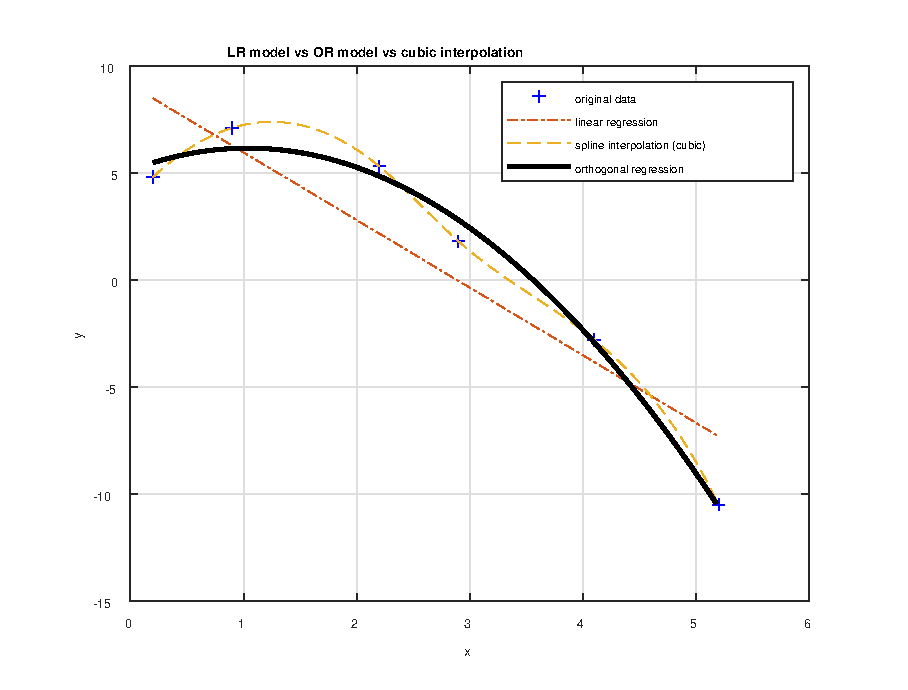
\includegraphics[width=\maxwidth{56.196688409433015em}]{figure_1.eps}
\end{center}

\begin{par}
\begin{flushleft}
Indeed, data fits so much better compared with the linear regression. Additionally, we have compared these values with a spline interpolation (i.e., the cubic interpolation of our points), and we can affirm that the error is acceptable.
\end{flushleft}
\end{par}


\label{H_B12D4B25}
\matlabheading{Exercise 2}

\begin{par}
\begin{flushleft}
Using the data from the file \texttt{svm\_complejo.txt} the following is requested: 
\end{flushleft}
\end{par}

\begin{par}
\begin{flushleft}
    a) Represent the data to try to identify a suitable kernel function. 
\end{flushleft}
\end{par}

\begin{par}
\begin{flushleft}
    b) With the available software (no need to program it), attempt to test different kernel functions to solve the classification problem.
\end{flushleft}
\end{par}


\label{H_0FCE7F48}
\matlabheadingtwo{Solution}


\label{H_C62820E9}
\matlabheadingthree{a) Represent the data to try to identify a suitable kernel function. }

\begin{par}
\hfill \break
\end{par}

\begin{matlabcode}
clear; clc
data = readtable('svm_complejo.csv','Delimiter',';');
x1 = data.x1; x2 = data.x2; y = data.y; X = [x1,x2];
data
\end{matlabcode}
\begin{matlabtableoutput}
{
\begin{tabular} {|c|c|c|c|}\hline
\mlcell{ } & \mlcell{x1} & \mlcell{x2} & \mlcell{y} \\ \hline
\mlcell{1} & \mlcell{2} & \mlcell{115} & \mlcell{1} \\ \hline
\mlcell{2} & \mlcell{3.5000} & \mlcell{105} & \mlcell{1} \\ \hline
\mlcell{3} & \mlcell{4} & \mlcell{130} & \mlcell{1} \\ \hline
\mlcell{4} & \mlcell{4.5000} & \mlcell{125} & \mlcell{1} \\ \hline
\mlcell{5} & \mlcell{5} & \mlcell{125} & \mlcell{1} \\ \hline
\mlcell{6} & \mlcell{6} & \mlcell{110} & \mlcell{1} \\ \hline
\mlcell{7} & \mlcell{7.5000} & \mlcell{109} & \mlcell{1} \\ \hline
\mlcell{8} & \mlcell{8} & \mlcell{105} & \mlcell{1} \\ \hline
\mlcell{9} & \mlcell{7.6000} & \mlcell{130} & \mlcell{1} \\ \hline
\mlcell{10} & \mlcell{7.8000} & \mlcell{130} & \mlcell{1} \\ \hline
\mlcell{11} & \mlcell{8.1000} & \mlcell{180} & \mlcell{1} \\ \hline
\mlcell{12} & \mlcell{8.3000} & \mlcell{190} & \mlcell{1} \\ \hline
\mlcell{13} & \mlcell{8.1000} & \mlcell{180} & \mlcell{1} \\ \hline
\mlcell{14} & \mlcell{2.5000} & \mlcell{130} & \mlcell{-1} \\ \hline
\mlcell{15} & \mlcell{3} & \mlcell{145} & \mlcell{-1} \\ \hline
\mlcell{16} & \mlcell{4} & \mlcell{150} & \mlcell{-1} \\ \hline
\mlcell{17} & \mlcell{4.5000} & \mlcell{160} & \mlcell{-1} \\ \hline
\mlcell{18} & \mlcell{4.7000} & \mlcell{180} & \mlcell{-1} \\ \hline
\mlcell{19} & \mlcell{5} & \mlcell{125} & \mlcell{-1} \\ \hline
\mlcell{20} & \mlcell{5.1000} & \mlcell{122} & \mlcell{-1} \\ \hline
\mlcell{21} & \mlcell{5.3000} & \mlcell{129} & \mlcell{-1} \\ \hline
\mlcell{22} & \mlcell{5.9000} & \mlcell{180} & \mlcell{-1} \\ \hline
\mlcell{23} & \mlcell{6.1000} & \mlcell{190} & \mlcell{-1} \\ \hline
\mlcell{24} & \mlcell{8.9000} & \mlcell{125} & \mlcell{-1} \\ \hline
\mlcell{25} & \mlcell{9} & \mlcell{180} & \mlcell{-1} \\ \hline
\mlcell{26} & \mlcell{9.1000} & \mlcell{130} & \mlcell{-1} \\ \hline
\mlcell{27} & \mlcell{9.3000} & \mlcell{190} & \mlcell{-1} \\ \hline
\mlcell{28} & \mlcell{9.5000} & \mlcell{160} & \mlcell{-1} \\ 
\hline
\end{tabular}
}
\end{matlabtableoutput}
\begin{matlabcode}
clf
figure(1)
gscatter(x1,x2,y)
grid on
xlabel('x_1')
ylabel('x_2')
\end{matlabcode}
\begin{center}
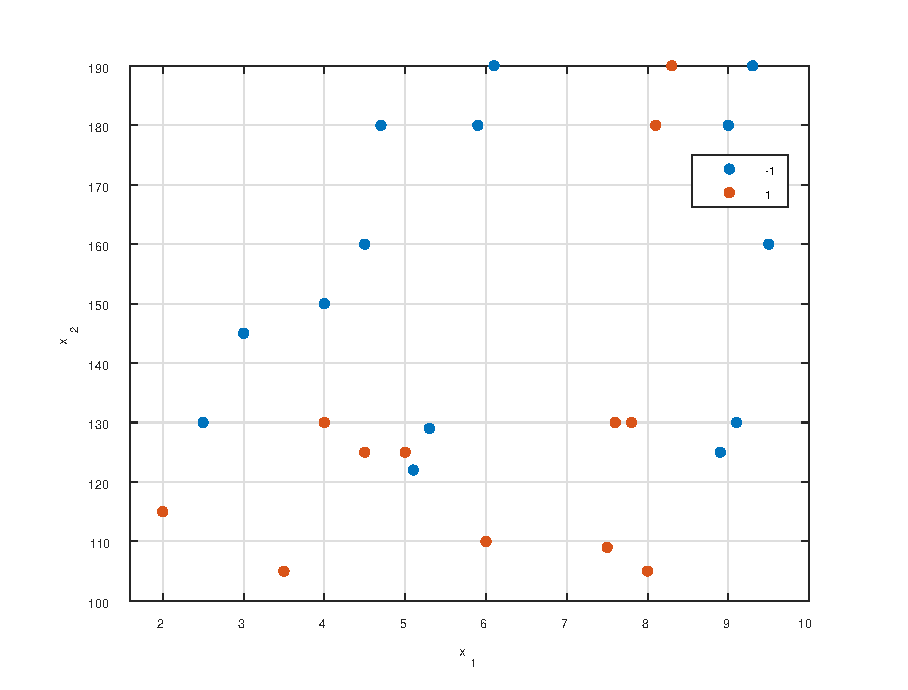
\includegraphics[width=\maxwidth{56.196688409433015em}]{figure_2.eps}
\end{center}

\begin{par}
\begin{flushleft}
Graphically, we can see that it does not exist a linear discriminant. It also seems that data can not be fitted easily to a polynomial curve. As for using a sigmoid-based kernel, it would be a good approximation although it would present some underfitting. 
\end{flushleft}
\end{par}

\begin{par}
\begin{flushleft}
So, since in general the groups are not too mixed with each other and there seems to be a certain distance between the different classes, we think that the best option will be to use a \textbf{Gaussian kernel} (although we cannot guarantee a priori that it fits perfectly or that tend to overfitting).
\end{flushleft}
\end{par}

\begin{par}
\begin{flushleft}
In any case, we are going to do an analysis based on all the kernel types and we will comment on them later.
\end{flushleft}
\end{par}


\label{H_6BF079EA}
\matlabheadingthree{b) With the available software (no need to program it), attempt to test different kernel functions to solve the classification problem.}

\begin{par}
\begin{flushleft}
As a first approach, we will try with the linear kernel. Then:
\end{flushleft}
\end{par}


\begin{itemize}
\setlength{\itemsep}{-1ex}
   \item{\begin{flushleft} \textbf{Linear Kernel} \end{flushleft}}
\end{itemize}

\begin{matlabcode}
model2 = fitcsvm(X, y, "KernelFunction", "linear");
\end{matlabcode}

\begin{par}
\begin{flushleft}
Our discriminant is given by the beta coefficients
\end{flushleft}
\end{par}

\begin{matlabcode}
w = model2.Beta;
b = model2.Bias;
kx1 = min(X(:,1)):0.1:max(X(:,1));
kx2 = (-w(1) * kx1 - b)/w(2); 

clf
figure(2)
plot(kx1, kx2, 'k', 'LineWidth', 2);
hold on;
h(1:2) = gscatter(X(:,1),X(:,2),y);
h(3) = plot(X(model2.IsSupportVector,1),...
    X(model2.IsSupportVector,2),'go','MarkerSize',10, 'LineWidth',1);
title('SVM with linear kernel')
grid on
legend('Separator', 'Group 1', 'Group 2','Support vector','Location','Best')
hold off;
\end{matlabcode}
\begin{center}
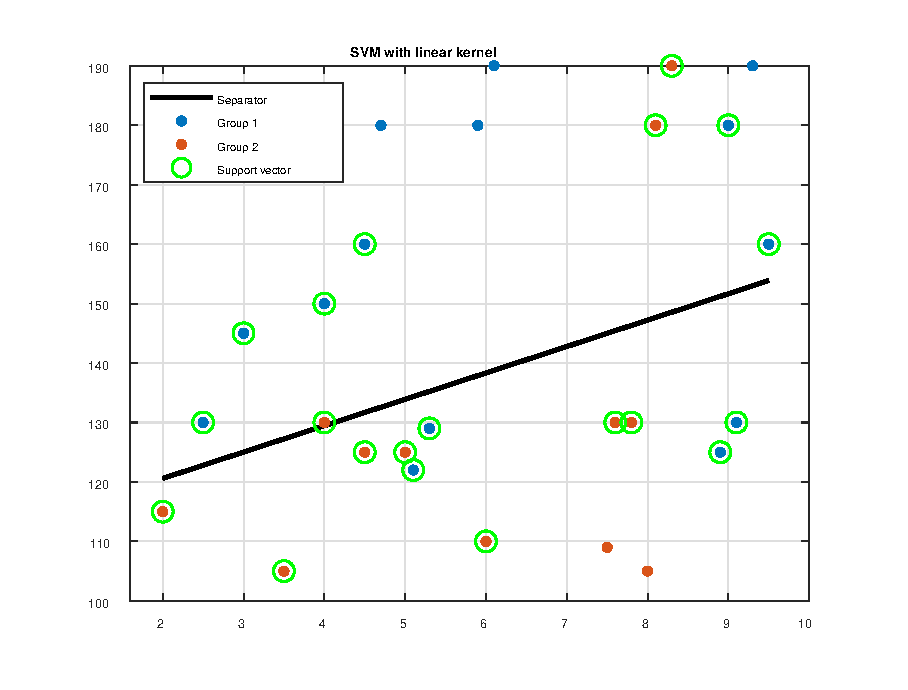
\includegraphics[width=\maxwidth{56.196688409433015em}]{figure_3.eps}
\end{center}

\begin{par}
\begin{flushleft}
\textbf{Results}: 2 points in group 1 misclassified; 5 points in group 2 misclassified. This is, indeed, a very bad result, specially for the second class.
\end{flushleft}
\end{par}


\begin{itemize}
\setlength{\itemsep}{-1ex}
   \item{\begin{flushleft} \textbf{Polynomial Kernel} \end{flushleft}}
\end{itemize}

\begin{par}
\begin{flushleft}
We will try with the simpler firstly, degree 2
\end{flushleft}
\end{par}

\begin{matlabcode}
model2 = fitcsvm(X, y, 'KernelFunction', 'polynomial', 'PolynomialOrder', 2);
sv = model2.SupportVectors;
% Grid
[xGrid, yGrid] = meshgrid(linspace(min(X(:, 1)), max(X(:, 1)), 1000), ...
                          linspace(min(X(:, 2)), max(X(:, 2)), 1000));
gridPoints = [xGrid(:), yGrid(:)];
predLabels = predict(model2, gridPoints);
figure;
gscatter(X(:, 1), X(:, 2), y);
hold on
contour(xGrid,yGrid,reshape(predLabels, size(xGrid)), 'k', 'LineWidth', 2);
plot(sv(:, 1), sv(:, 2), 'go', 'MarkerSize', 10, 'LineWidth', 1);
title('SVM Model with Polynomial Kernel (Degree 2)');
xlabel('x1');
ylabel('x2');
legend('Class -1', 'Class 1', 'Separator', 'Support Vectors');
hold off;
\end{matlabcode}
\begin{center}
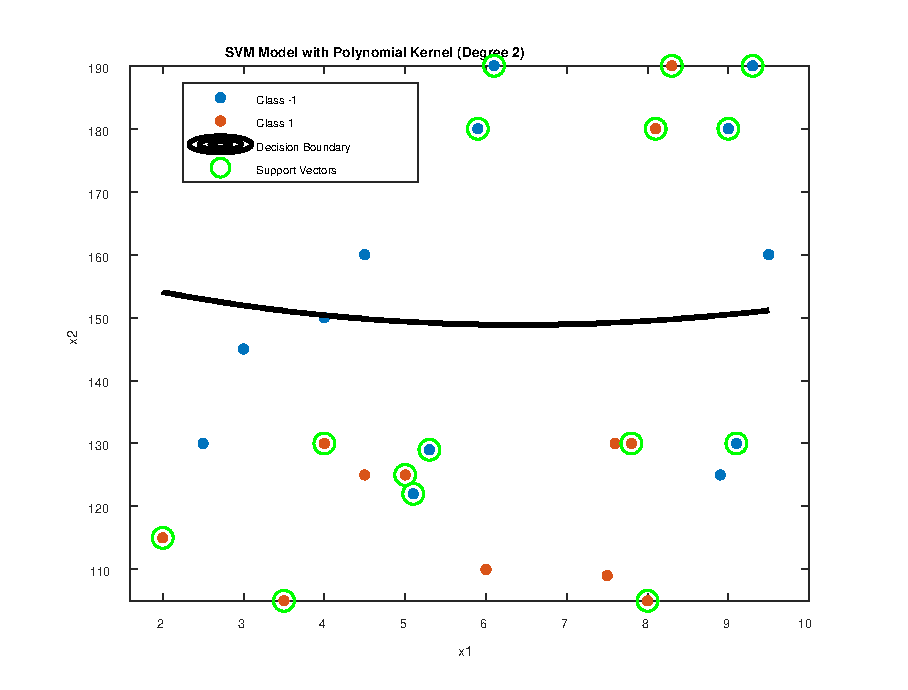
\includegraphics[width=\maxwidth{56.196688409433015em}]{figure_4.eps}
\end{center}

\begin{par}
\begin{flushleft}
As we can see, \textbf{this method does not fit our data at all}. If we try to use another polynomial kernel with higher degree, we cannot perform it.
\end{flushleft}
\end{par}


\begin{itemize}
\setlength{\itemsep}{-1ex}
   \item{\begin{flushleft} \textbf{Gaussian kernel} \end{flushleft}}
\end{itemize}

\begin{matlabcode}
model3 = fitcsvm(X, y, "KernelFunction","rbf"); % rbf states for radial basis function
[x1Grid, x2Grid] = meshgrid(linspace(min(X(:, 1)), max(X(:, 1)), 1000), ...
                          linspace(min(X(:, 2)), max(X(:, 2)), 1000));
xGrid = [x1Grid(:),x2Grid(:)];
[~,scores1] = predict(model3,xGrid); % The scores

figure(3)
contour(x1Grid,x2Grid,reshape(scores1(:,2),size(x1Grid)),[0 0],'k','LineWidth',2);
hold on
gscatter(X(:,1),X(:,2),y);
plot(X(model2.IsSupportVector,1),...
    X(model2.IsSupportVector,2),'go','MarkerSize', 10, 'LineWidth', 1);
title('SVM with gaussian kernel')
legend({'Separator','Group 1','Group 2','Support Vectors'},'Location','Best');
hold off
\end{matlabcode}
\begin{center}
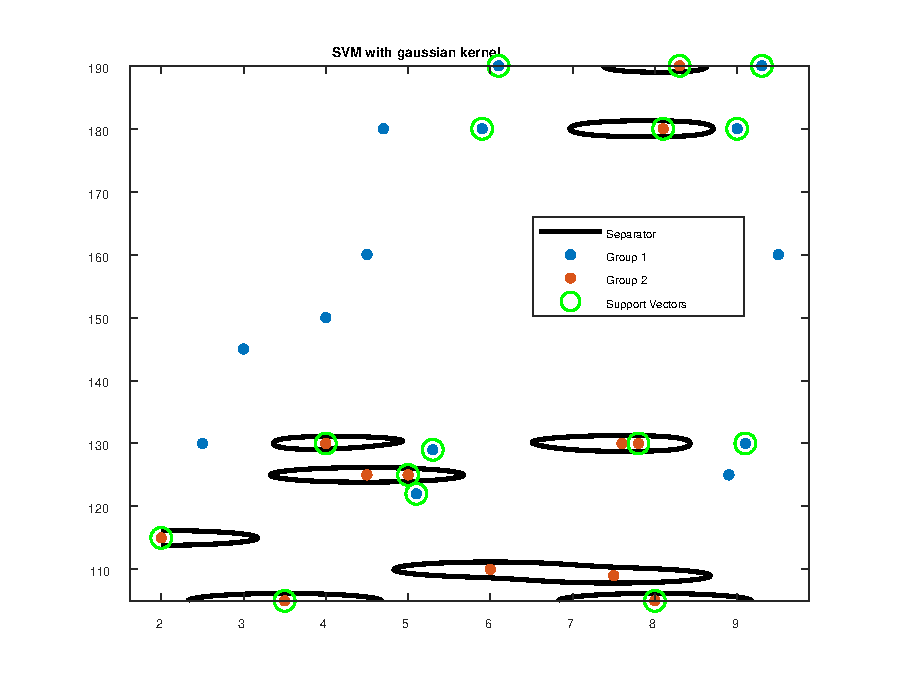
\includegraphics[width=\maxwidth{56.196688409433015em}]{figure_5.eps}
\end{center}

\begin{par}
\begin{flushleft}
This method fits with our data, but it seems like the algorithm has generated a higher number of ellipsoids than expected. Furthermore, ellipsoids have a very small area. In other words, the SVM algorithm has overfitted (a problem that is named \textit{curse of the dimensionality}).
\end{flushleft}
\end{par}

\begin{par}
\begin{flushleft}
A way to solve this is applying cross-validation (but it is not object of this practice). Then, a model can be selected depending on information criterion such as BIC or AIC values (but again, this is not the objective of this practice). The code for the cross validation is on \hyperref[H_10E9D3A0]{annexes}.
\end{flushleft}
\end{par}

\begin{matlabcode}
cross_val_svm(y,X,4,'rbf') % this is a function created by me which makes the cross-validation process on n-folds.
\end{matlabcode}
\begin{center}
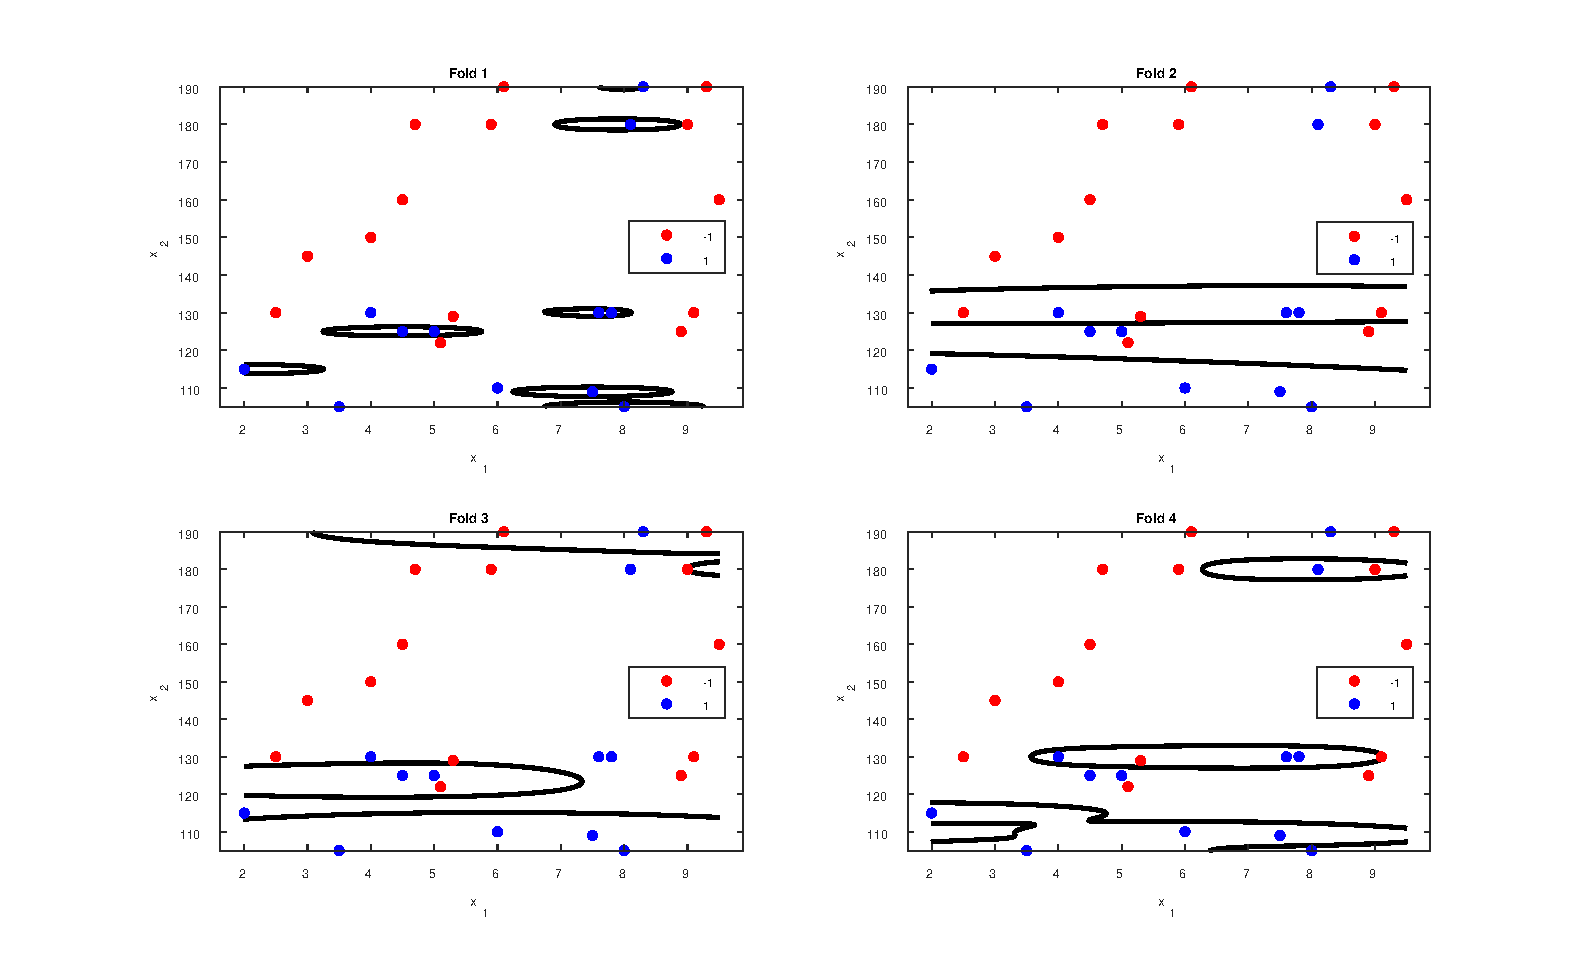
\includegraphics[width=\maxwidth{100.35122930255896em}]{figure_6.eps}
\end{center}

\begin{par}
\begin{flushleft}
\textbf{Conclusion: the model which best suits for this use case is the Gaussian-kernel-based model.}
\end{flushleft}
\end{par}


\label{H_59140F30}
\matlabheading{\textbf{Annexes}}

\label{H_10E9D3A0}
\matlabheadingtwo{\textbf{Cross Validation for SVM function}}

\begin{matlabcode}
function [] = cross_val_svm(y,X,n,svm_method)
%% Cross-validation of a svm model.

% Create a cross-validation partition
cvp = cvpartition(y, 'KFold', n); % 5-fold cross-validation

% Initialize an array to store the trained SVM models
models = cell(cvp.NumTestSets, 1);

% Create a new figure and specify its size
fig = figure('Position', [100, 100, 1000, 600]);

for i = 1:cvp.NumTestSets
    % Split the data into training and testing sets
    trainIdx = cvp.training(i);
    testIdx = cvp.test(i);
    X_train = X(trainIdx, :);
    y_train = y(trainIdx);
    X_test = X(testIdx, :);
    y_test = y(testIdx);

    % Train the SVM model with an RBF kernel
    SVMModel = fitcsvm(X_train, y_train, 'KernelFunction', svm_method, 'BoxConstraint', 1, 'KernelScale', 'auto');

    % Store the trained model
    models{i} = SVMModel;
    
    if mod(n,2)==1
        m = floor(n/2) + 1;
    else
        m = n/2;
    end
       
    % Create subplots with larger size
    subplot(2, m, i, 'Parent', fig); % Adjust the subplot arrangement as needed

    % Create a grid for plotting
    x1 = linspace(min(X(:, 1)), max(X(:, 1)), 3000);
    x2 = linspace(min(X(:, 2)), max(X(:, 2)), 3000);
    [X1, X2] = meshgrid(x1, x2);
    XGrid = [X1(:), X2(:)];

    % Calculate scores for the grid points
    scores = predict(SVMModel, XGrid);
    scores = reshape(scores, size(X1));

    % Plot the decision boundary
    contour(x1, x2, scores, [0, 0], 'k', 'LineWidth', 2);
    hold on;

    % Plot the data points
    gscatter(X(:, 1), X(:, 2), y, 'rb');
    
    title(['Fold ', num2str(i)]);
    xlabel('x_1');
    ylabel('x_2');
end
end
\end{matlabcode}

\end{document}
